%3-3-CW-isosceles.tex

\documentclass[12pt, oneside]{article}
\usepackage[letterpaper, margin=1in, headsep=0.5in]{geometry}
\usepackage[english]{babel}
\usepackage[utf8]{inputenc}
\usepackage{amsmath}
\usepackage{amsfonts}
\usepackage{amssymb}
\usepackage{tikz}
\usetikzlibrary{quotes, angles}
\usepackage{graphicx}

\usepackage{fancyhdr}
\pagestyle{fancy}
\fancyhf{}
\rhead{\thepage \\Name: \hspace{1.5in}.\\}
\lhead{BECA / Dr. Huson / 10th Grade Geometry\\* 15 November 2018}

\renewcommand{\headrulewidth}{0pt}

\begin{document}
\subsubsection*{Classwork: base theorem}
\begin{enumerate}

  \item Given $\triangle ABC$.

  \item Given $\triangle DEF$.\\[0.5cm]
    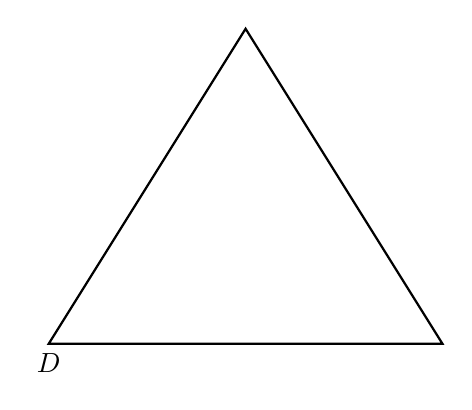
\begin{tikzpicture}
      \draw [-, thick] (0,0) node[below]{$D$}--
        (5,0)--(2.5,4)--cycle;
     \end{tikzpicture}

\newpage
    \item Given circle $Z$

    \item Given circle $O$
      \begin{enumerate}
        \item part 1
        \item part 2
        \item part3
      \end{enumerate}
    
    \item Why do we write down theorems?

\end{enumerate}
\end{document}
